% ==============================================================================
% FRAME 1 : SRAM
% ==============================================================================

\begin{frame}{Stockage des données \textit{massives}}
  \begin{columns}[T]
    \begin{column}{0.5\textwidth}
      \begin{itemize}
        \item Les \textbf{registres} stockent les données.
        \begin{itemize}
          \item \textbf{Rappel} : \textit{registre} =  \textit{Bascule D}.
        \end{itemize}
        \item Mais ils ont un coût élevé :
        \begin{itemize}
          \item Environ 10 portes logiques pour 1 bascule D.
          \item Prohibitif pour de grandes qualité de données.
          \item Nécessité d'autres technologies pour ce stockage massif.
        \end{itemize}
        \item Objectif : se rapprocher de la manipulation logicielle de \textit{tableaux}
          \begin{itemize}
            \item \texttt{int t[1000]=\{23,18,5,-4,...\};}
            \item \texttt{t[123] = -47; // écriture}
            \item \texttt{int x= 42 * t[2]; // lecture}
          \end{itemize}
        \end{itemize}
    \end{column}
    \begin{column}{0.5\textwidth}
      \centering
      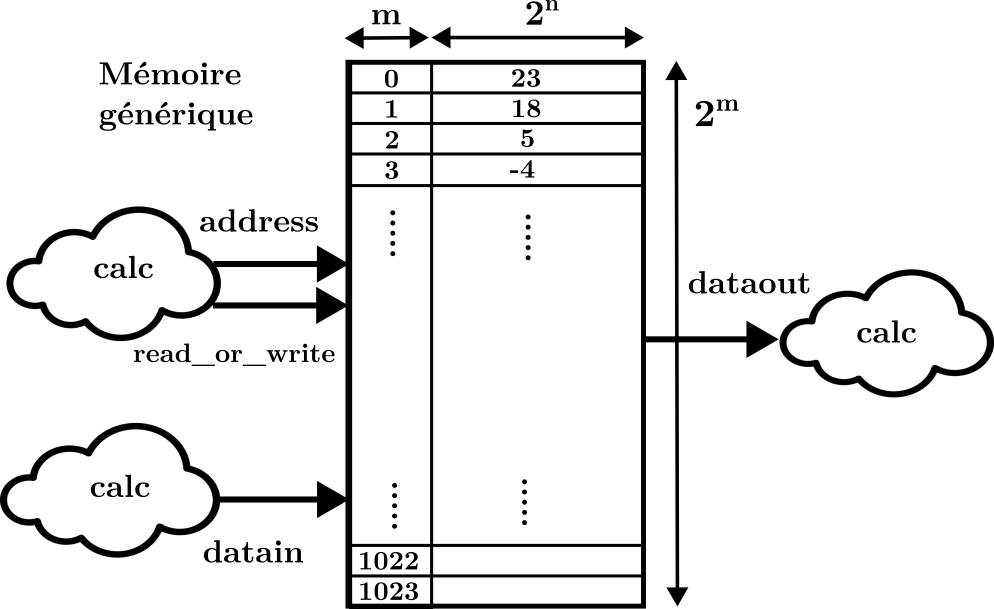
\includegraphics[scale=0.29]{./images/memory.png}
    \end{column}
  \end{columns}
\end{frame}

\begin{frame}{Mémoire SRAM (Static Random Access Memory)}
  \small
    \begin{columns}[T]
        \begin{column}{0.55\textwidth}
            \textbf{Principe de la cellule (6T)} :
            \begin{itemize}
                \item Bistable à 6 transistors (2 inverseurs couplés + 2 transistors d'accès).
                \item \textbf{Statique} : conserve l'information tant qu'elle est alimentée (pas de rafraîchissement).
                \item Très rapide, mais faible densité (surface silicium importante).
            \end{itemize}

            \vspace{0.3cm}
            \textbf{Signaux de commande typiques} :
            \begin{itemize}
                \item \texttt{ADDR} : Bus d'adresse (sélectionne la ligne via \textit{Word Line} et la colonne).
                \item \texttt{CS} (\textit{Chip Select}) : Activation de la puce.
                \item \texttt{WE} (\textit{Write Enable}) : \texttt{1} pour écriture, \texttt{0} pour lecture.
                \item \texttt{OE} (\textit{Output Enable}) : Active les buffers de sortie.
                \item \texttt{D\textsubscript{in}} / \texttt{D\textsubscript{out}} : Bus de données.
            \end{itemize}
        \end{column}

        \begin{column}{0.45\textwidth}
            \centering
            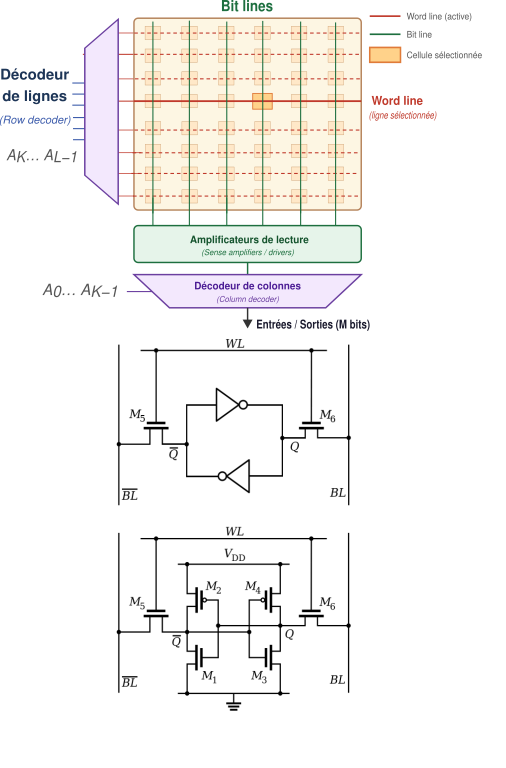
\includegraphics[scale=0.39]{./images/sram_cellule_6t.png}
        \end{column}
    \end{columns}
\end{frame}

% ==============================================================================
% FRAME 2 : DRAM
% ==============================================================================
\begin{frame}{Mémoire DRAM (Dynamic Random Access Memory)}
    \small
    \begin{columns}[T]
        \begin{column}{0.55\textwidth}
            \textbf{Principe de la cellule (1T1C)} :
            \begin{itemize}
                \item 1 Transistor d'accès + 1 Condensateur de stockage.
                \item \textbf{Dynamique} : la charge du condensateur fuit, nécessitant un \textbf{rafraîchissement périodique} (typ. toutes les 64 ms).
                \item Haute densité, faible coût par bit, mais lente.
            \end{itemize}

            \vspace{0.3cm}
            \textbf{Signaux de commande et usage} :
            \begin{itemize}
                \item \texttt{RAS} (\textit{Row Address Strobe})
                \begin{itemize}
                  \item Valide l'adresse de ligne (ouvre la rangée).
                \end{itemize}
                \item \texttt{CAS} (\textit{Column Address Strobe}) :
                \begin{itemize}
                  \item Valide l'adresse de colonne (sélectionne le mot).
                \end{itemize}
                \item \texttt{WE} : \texttt{0} pour écriture, \texttt{1} pour lecture (e.g).
                \item \texttt{DQ} : Bus de données bidirectionnel (Data In/Out multiplexé).
            \end{itemize}
        \end{column}

        \begin{column}{0.45\textwidth}
            \centering
            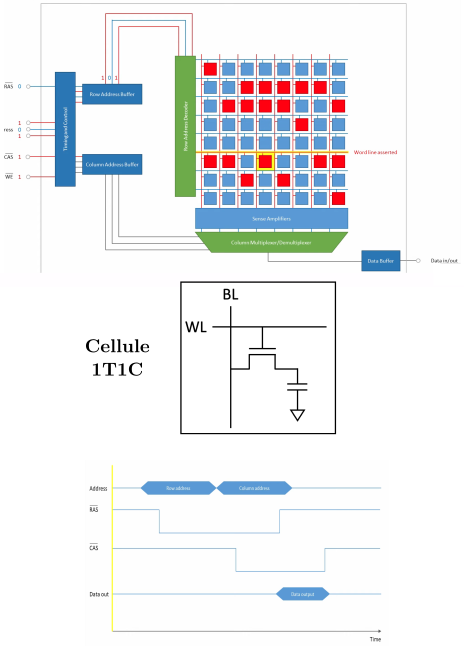
\includegraphics[scale=0.45]{./images/dram_cellule_1t1c.png}
        \end{column}
    \end{columns}
\end{frame}

% ==============================================================================
% FRAME 3 : COMPARAISON ET HIÉRARCHIE
% ==============================================================================
\begin{frame}{Comparaison et Utilisation dans la Hiérarchie Mémoire}
    \small
    \begin{table}
      \centering
      \renewcommand{\arraystretch}{1.3}
      \begin{tabular}{lcc}
        \toprule
        \textbf{Caractéristique} & \textbf{SRAM} & \textbf{DRAM} \\
        \midrule
        \textbf{Cellule} & 6 transistors (6T) & 1T + 1 Condensateur (1T1C) \\
        \textbf{Densité} & Faible & Élevée \\
        \textbf{Vitesse d'accès} & Très rapide (\(\sim\) 1-10 ns) & Rapide (\(\sim\) 10-50 ns) \\
        \textbf{Rafraîchissement} & Non requis & Obligatoire (périodique) \\
        \textbf{Consommation} & Faible (en veille) & Moyenne (à cause du refresh) \\
        \textbf{Coût par bit} & Élevé & Faible \\
        \bottomrule
      \end{tabular}
    \end{table}

    \begin{columns}[T]
        \begin{column}{0.6\textwidth}
            \vspace{0.2cm}
            \textbf{Utilisation système typique} :
            \begin{itemize}
                \item \textbf{SRAM} : Mémoires Cache (L1, L2, L3), mémoires tampons, registres. Proche du cœur de processeur.
                \item \textbf{DRAM} : Mémoire principale du système (barrettes DDR4/DDR5). Gestion par un contrôleur mémoire dédié (MMC).
            \end{itemize}
        \end{column}

        \begin{column}{0.4\textwidth}
            \centering
            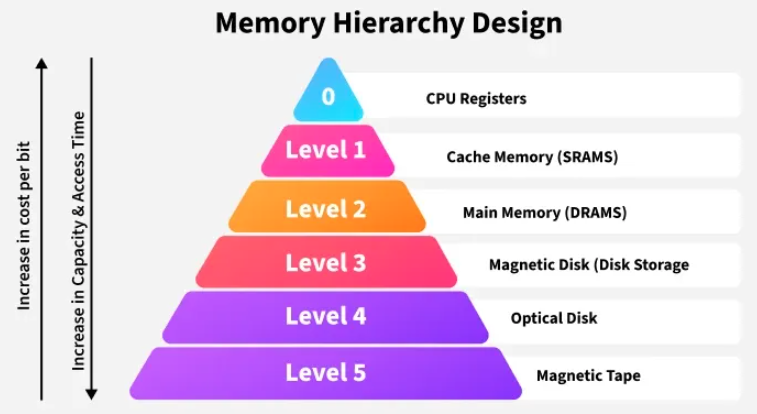
\includegraphics[scale=0.22]{./images/memory_hierarchy.png}
        \end{column}
    \end{columns}
\end{frame}
